\documentclass{beamer}
\usetheme[hideothersubsections]{AUTheme}
% \setbeamertemplate{caption}[numbered]
\setbeamertemplate{bibliography item}[text]%,
\setbeamertemplate{footline}[frame number]

\usepackage[scaled]{helvet}

\usepackage{url}

\usepackage{tikz,pgf}
\usetikzlibrary{arrows}

\usepackage{epstopdf}
\usepackage{siunitx}
\usepackage{amsmath}
\usepackage{graphicx,subfigure}
\usepackage[maxcitenames = 1, mincitenames=1,backend=bibtex]{biblatex}
\usepackage{multicol}
\usepackage{wrapfig}
% \usepackage{cutwin} % this is awful.
% \usepackage[utf8]{inputenc}
\usepackage{hypcap}
\usepackage{lipsum}
\usepackage[absolute,overlay]{textpos}
% \usepackage[sf,sl,outermarks]{titlesec}
\usepackage{caption}

\captionsetup[figure]{labelformat=empty}

\hyphenation{op-tical net-works semi-conduc-tor}



\AtBeginSection[] {
  \begin{frame}<beamer>
    \frametitle{Section Outline}
    \tableofcontents[currentsection,hideallsubsections]
  \end{frame}
}

\bibliography{../bib/master.bib} % problems here
\newcommand{\citeitem}[1]{[\emph{\Citeauthor*{#1}, \citeyear{#1} }]}

\title[DRTK Driver Assistance]{An On-Line Visual Driver Aid for\\ Safe and Precise Convoy Following in\\ Visibility-Impaired Conditions}
\author[]{Robert Cofield, Scott Martin, David Bevly}
\date{September , 2013} 

%%%%%%%%%%%%%%%%%%%%%%%%%%%%%%%%%%%%%%%%%%%%%%%%%%%%%%%%%%%%%%%%%%%%%%%%%%%%%%%%

\begin{document}

%% Title Slide %%
\frame{\titlepage}

%%%%%%%%%%%%%%%%
%% Motivation %%
%%%%%%%%%%%%%%%%

\section{Motivation}

  %% Military 
  \begin{frame}{Military Convoying}
    \begin{figure}
      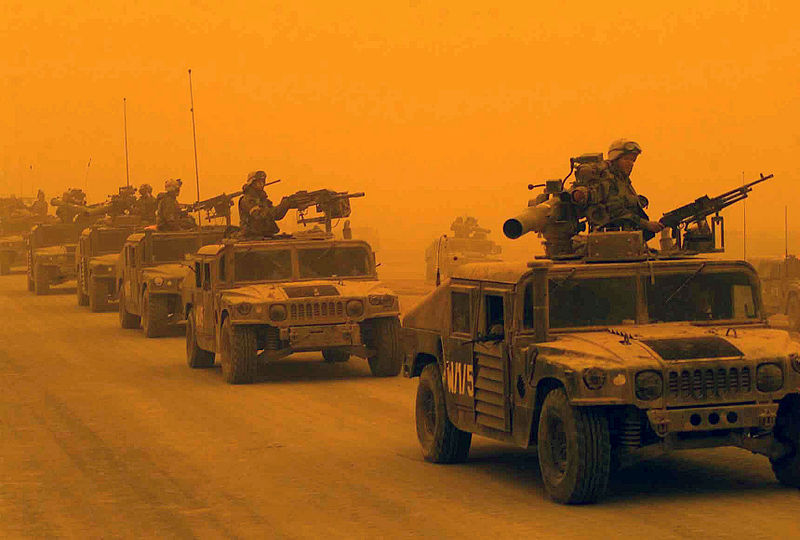
\includegraphics[width=5cm]{../graphics/convoy_sandstorm_orange.jpg}
      \vspace{-10pt}
      \caption{\tiny Source: \citeauthor{convoy_dust_orange}}
    \end{figure}
  \end{frame}


%%%%%%%%%%%%%%%%%%%%%%%%%%%%%%%%
%% Literature & Previous Work %%
%%%%%%%%%%%%%%%%%%%%%%%%%%%%%%%%

\section{Literature}

  \subsection{DRTK}

    %% brief explanation
    \begin{frame}{Dynamic Base Real-Time Kinematic GNSS}
      \begin{itemize}
        \item LAMBDA Integer-Fixing Method
      \end{itemize}
    \end{frame}

    %% discuss accuracy
    \begin{frame}{Errors in DRTK}
    \end{frame}

  \subsection{TDCP}

    %% brief explanation
    \begin{frame}{Time-Differenced Carrier Phase GNSS}
    \end{frame}

    %% discuss accuracy
    \begin{frame}{Errors in TDCP}
    \end{frame}

  \subsection{Virtual Path}

    %% discuss virtual leader & path summation
    \begin{frame}{Construction of Path}
      \begin{figure}
        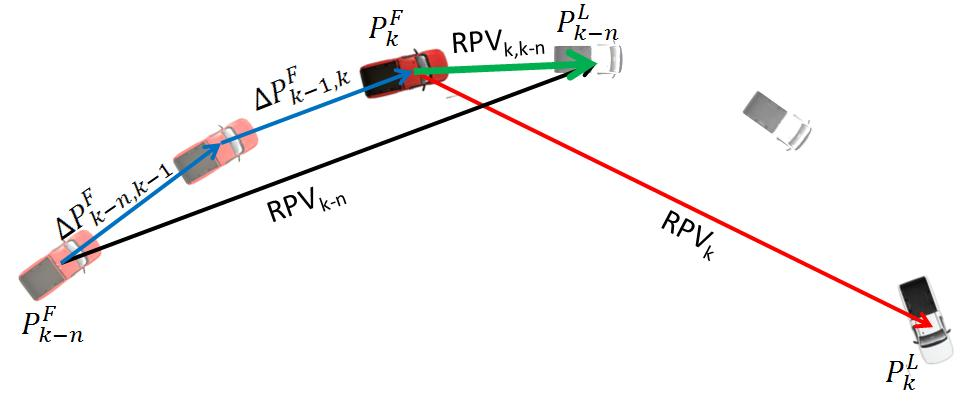
\includegraphics[width=10cm]{../graphics/path_algorithm.png}
      \end{figure}
    \end{frame}


%%%%%%%%%%%%%%%%%%%%%%%%%%%%%%%%%%%%
%% Presentation of final products %%
%%%%%%%%%%%%%%%%%%%%%%%%%%%%%%%%%%%%

\section{GUI}


  % Transition slide from Literature
  % Talk about waypoint following with Prowler
  \begin{frame}{Real-Time Implementation}
    \begin{minipage}{0.45\textwidth}
      \centering
      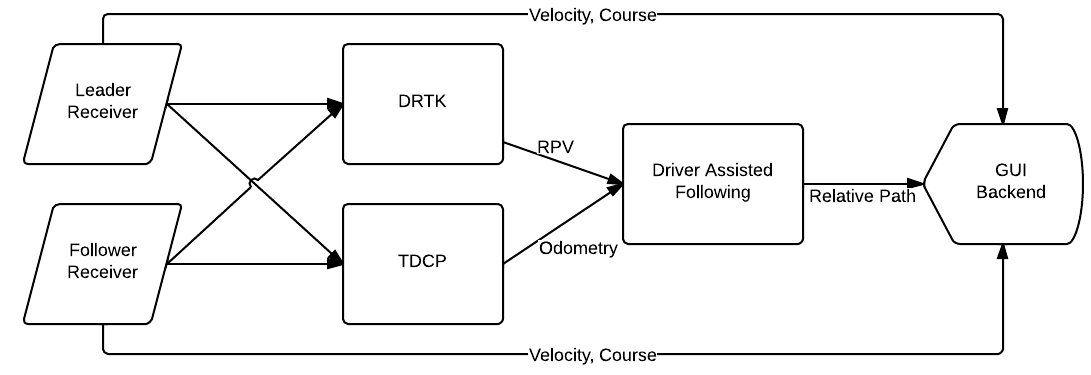
\includegraphics[width=\textwidth]{../graphics/data_algo.png}
    \end{minipage}
    \begin{minipage}{0.45\textwidth}
      \begin{itemize} \small
        \item DRTK, TDCP errors analyzed by splitting single antenna between 2 receivers
        \item Unmanned Following
        \item Waypoint-based control
        \item No intuitive method for quickly tuning algorithms \& visualizing errors
      \end{itemize}
    \end{minipage}
  \end{frame}

  %% ConOps
  \begin{frame}{Concept of Operation}
    \begin{figure}
      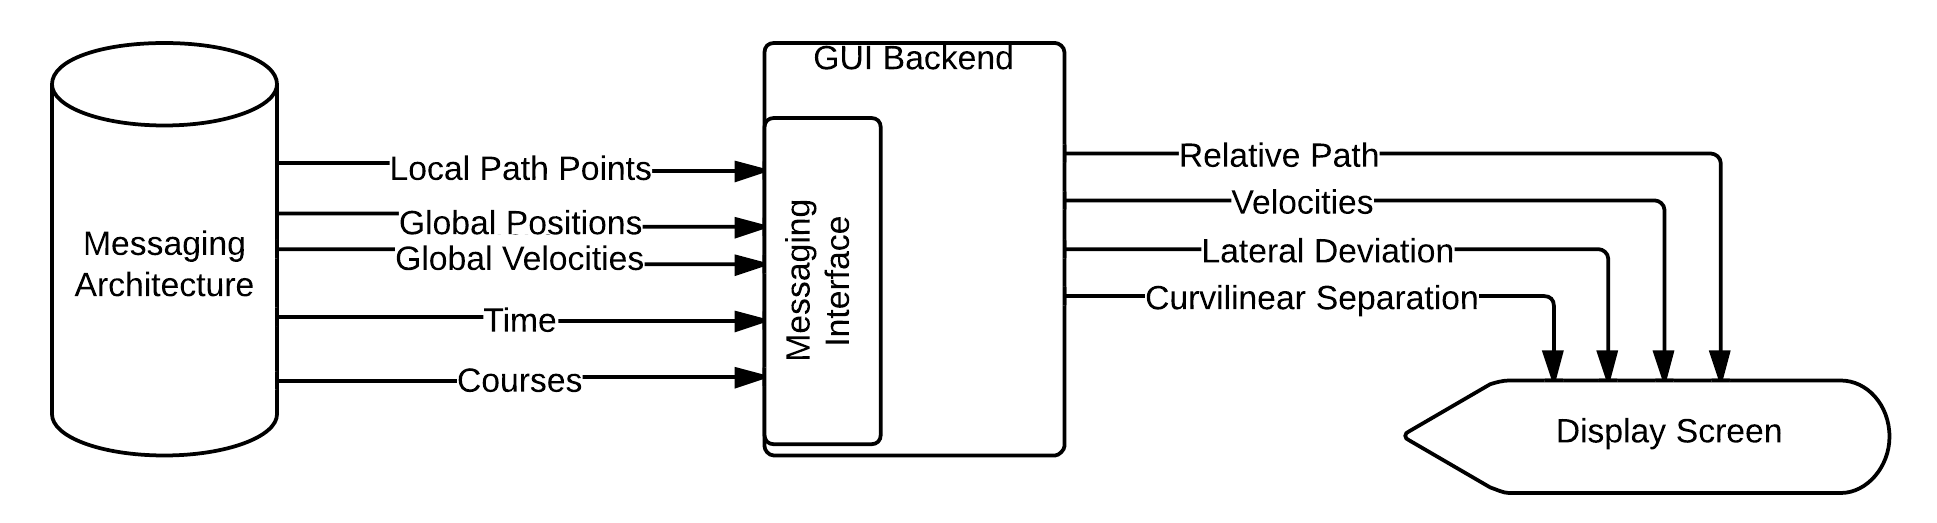
\includegraphics[width=0.8\textwidth]{../graphics/blackbox_flowchart.png}
    \end{figure}
    \begin{columns}  
      \begin{column}{0.5\textwidth}
        \footnotesize User inputs
        \begin{itemize} \footnotesize
          \item Critical alert values\\ ($\mu_{crit}~,~d_{crit}$)
          \item Warning alert values\\ ($\mu_{warn}$~,~$d_{warn}$)
        \end{itemize}
      \end{column}
      \begin{column}{0.5\textwidth}
        \footnotesize Relay to user
        \begin{itemize} \footnotesize
          \item Lateral path deviation alerts
          \item Path separation distance alerts
        \end{itemize}
      \end{column}
    \end{columns}
  \end{frame}


  %%% Qt GUI %%%%
  \subsection{Qt}

    % what led to simple GUI
    % mention SBIR?
    \begin{frame}{Initial Design Goals}
      \begin{itemize}
        \item
      \end{itemize}
    \end{frame}

    \begin{frame}{Qt-Based GUI --- Data Display}
      \begin{figure}[ht] \centering
        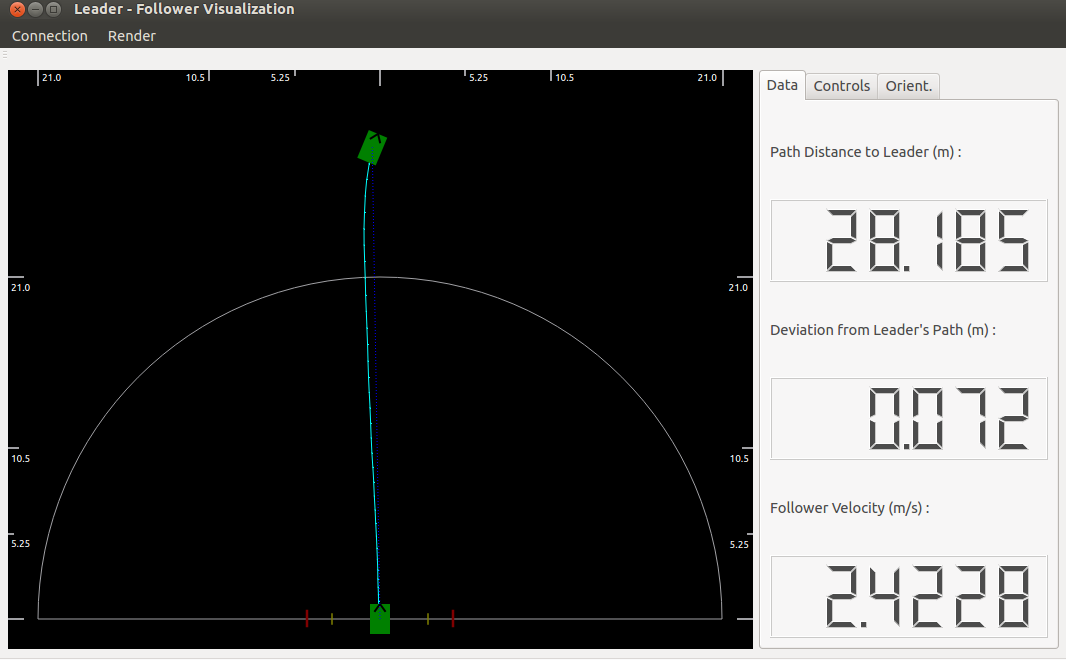
\includegraphics[width=4in] {../graphics/final_design_data.png}
        \caption{Qt GUI in normal operation} \label{fig:qt_data_display}
      \end{figure}
    \end{frame}

    \begin{frame}{Qt-Based GUI --- Controls}
      \begin{figure}[ht] \centering
        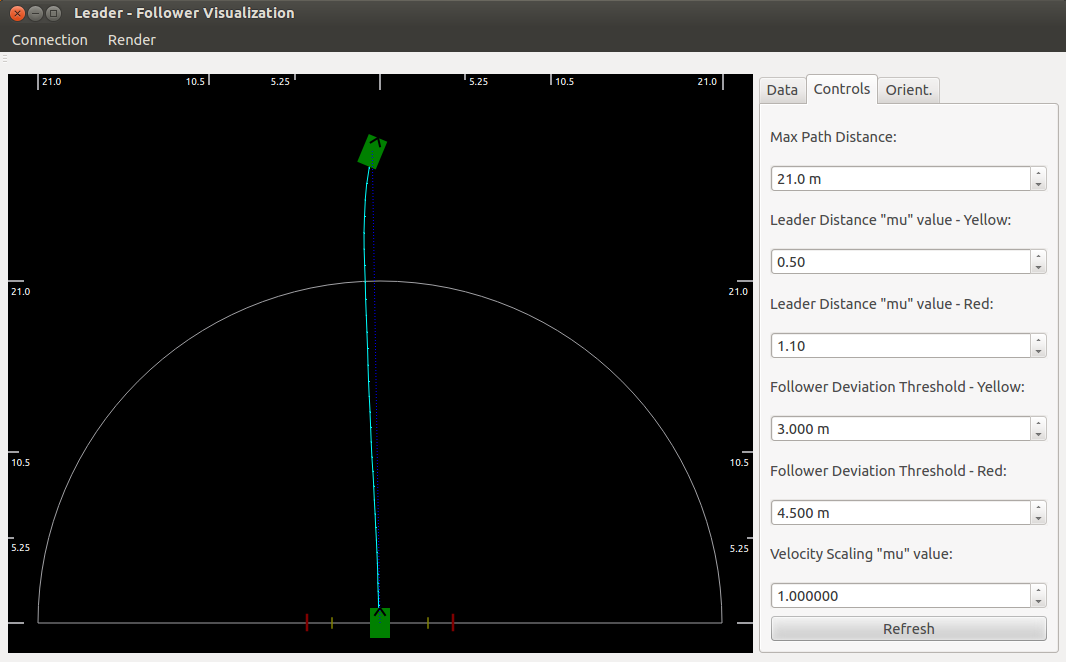
\includegraphics[width=4in] {../graphics/final_design_opts.png}
        \caption{Qt GUI displaying view control data} \label{fig:qt_controls}
      \end{figure}
    \end{frame}


  %%% Google Earth GUI %%%
  \subsection{Earth}

    \begin{frame}{Google Earth GUI --- Data Display}
    \end{frame}

    \begin{frame}{Google Earth GUI -- Controls}
      \begin{figure}
        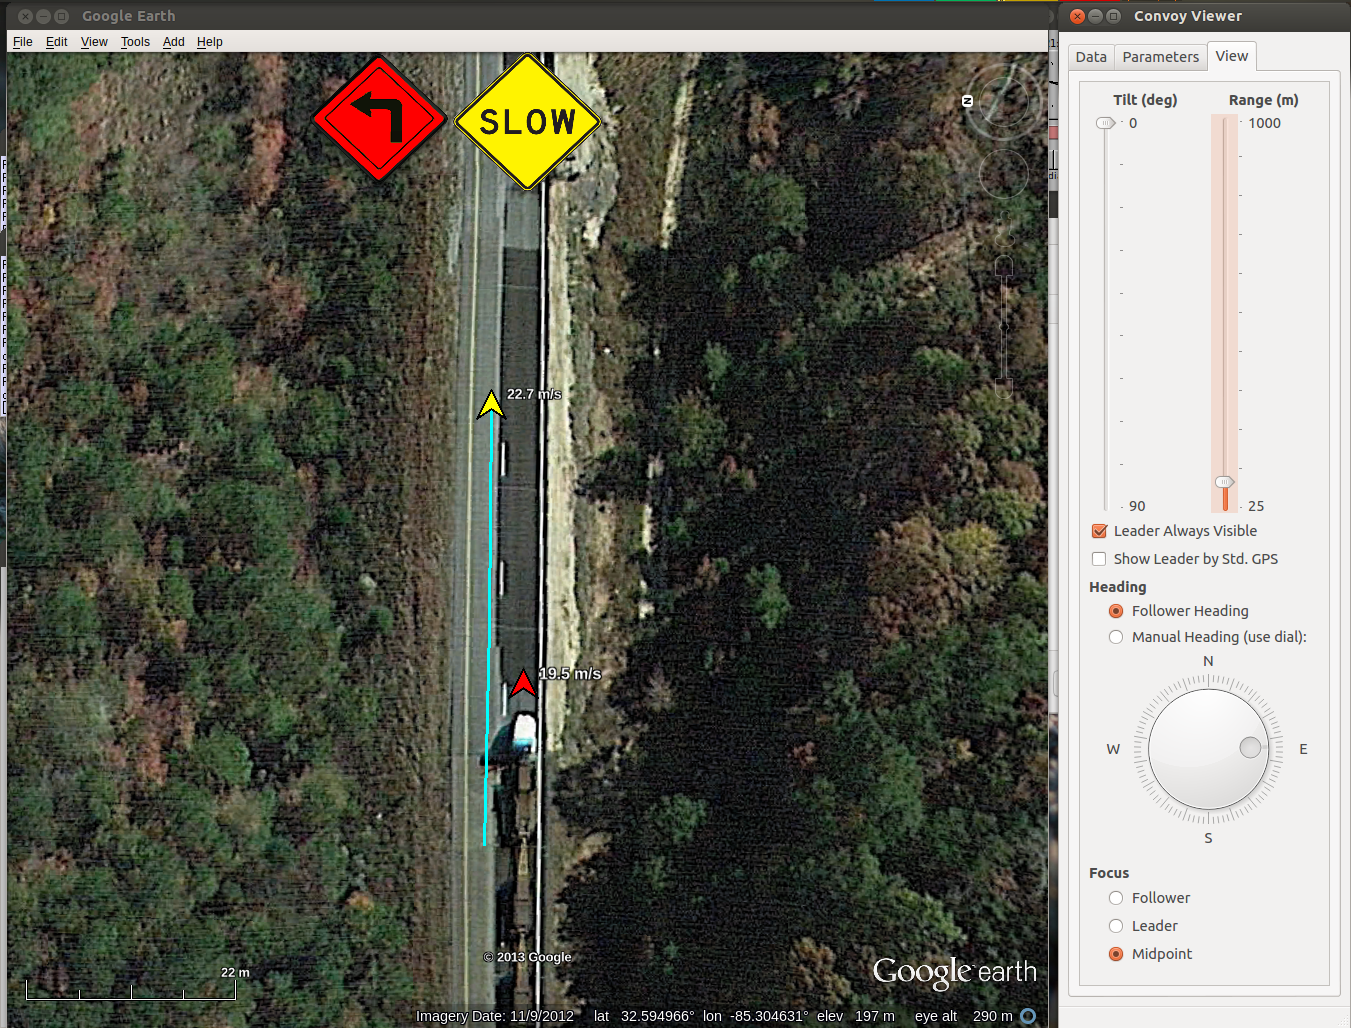
\includegraphics[width=0.9\textwidth]{../graphics/earth_slow.png}
      \end{figure}
    \end{frame}


  \subsection{Middleware}

    % talk about MOOS , etc
    \begin{frame}{Middleware}
    \end{frame}

    %% introduce interpolation
    \begin{frame}{Interpolation}
      \begin{figure}[ht] \centering
        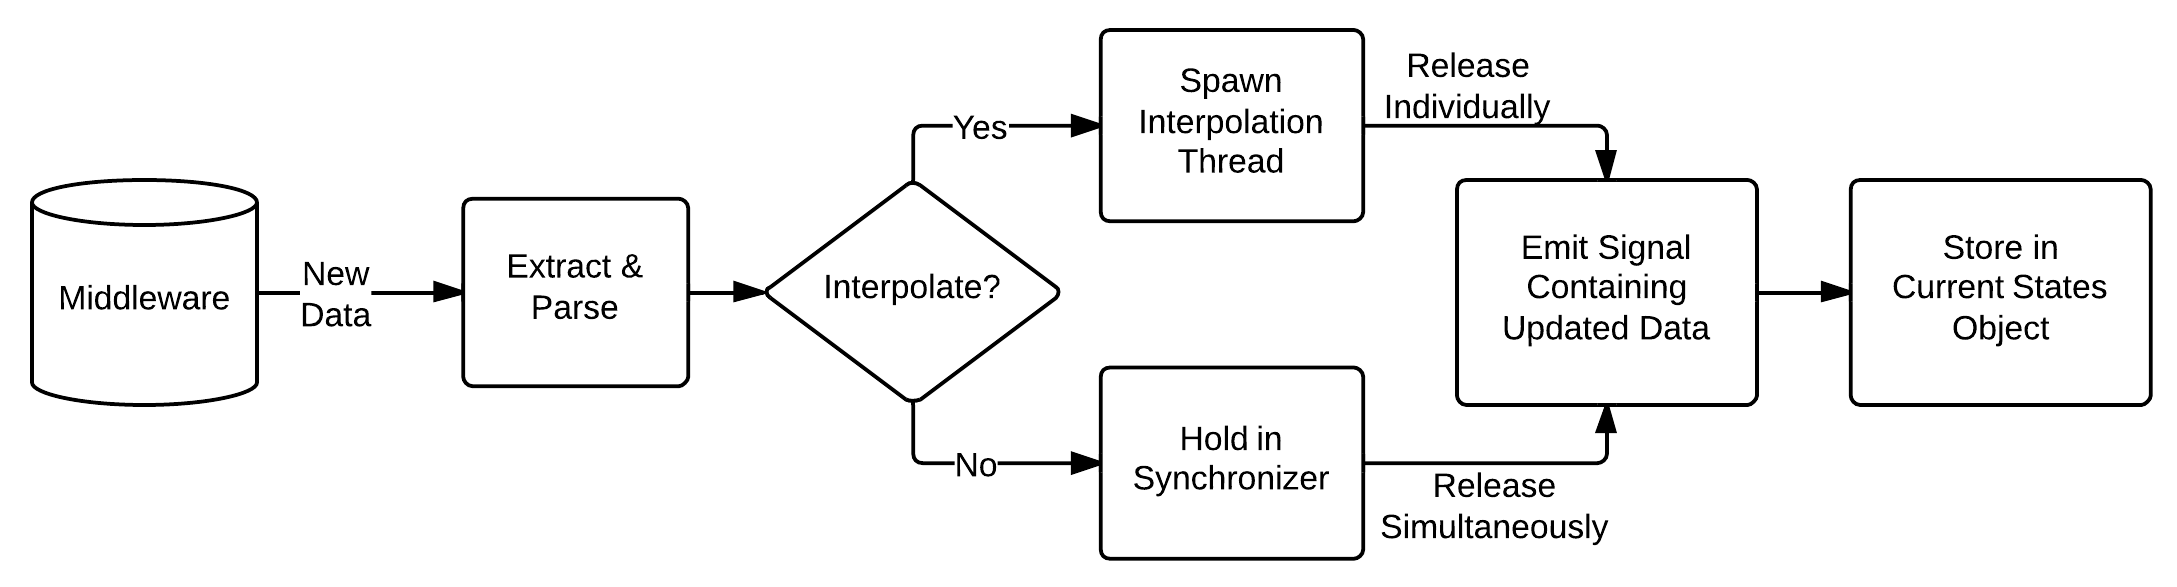
\includegraphics[width=5cm] {../graphics/middleware_diagram.png}
      \end{figure}
    \end{frame}


%%%%%%%%%%%%%%%%%%%%%%%%%%%%%%%%%%%
%% Tests that were run & Results %%
%%%%%%%%%%%%%%%%%%%%%%%%%%%%%%%%%%%

\section{Experimentation}

  \subsection{Hardware \& Setup}

    \begin{frame}{Hardware}
        \begin{minipage}{0.45\textwidth}
          \centering
          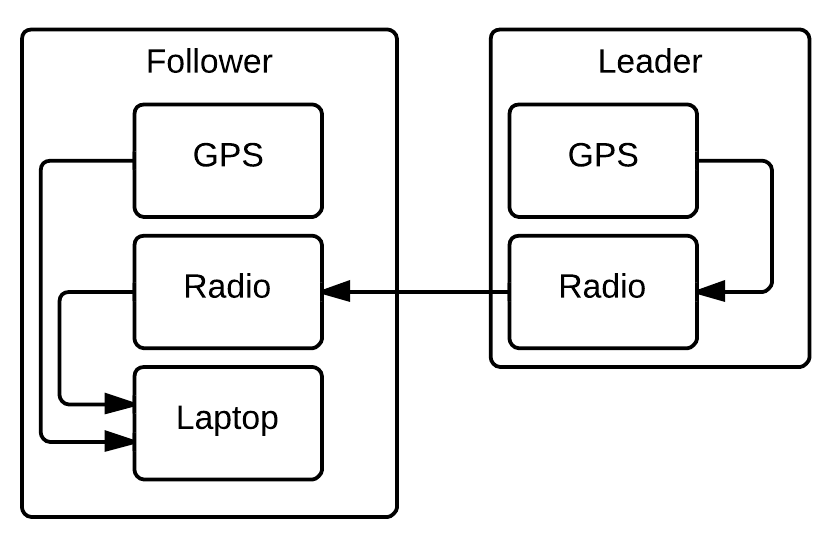
\includegraphics[width=4cm]{../graphics/hardware_flow.png}
        \end{minipage}
        \begin{minipage}{0.45\textwidth}
          \begin{itemize}
            \item Novatel Propak v3 (OEMV board) L1/L2
            \item Pinwheel Antenna
            \item Digi Extend 900 Mhz radio
          \end{itemize}
        \end{minipage}
        \begin{figure}
          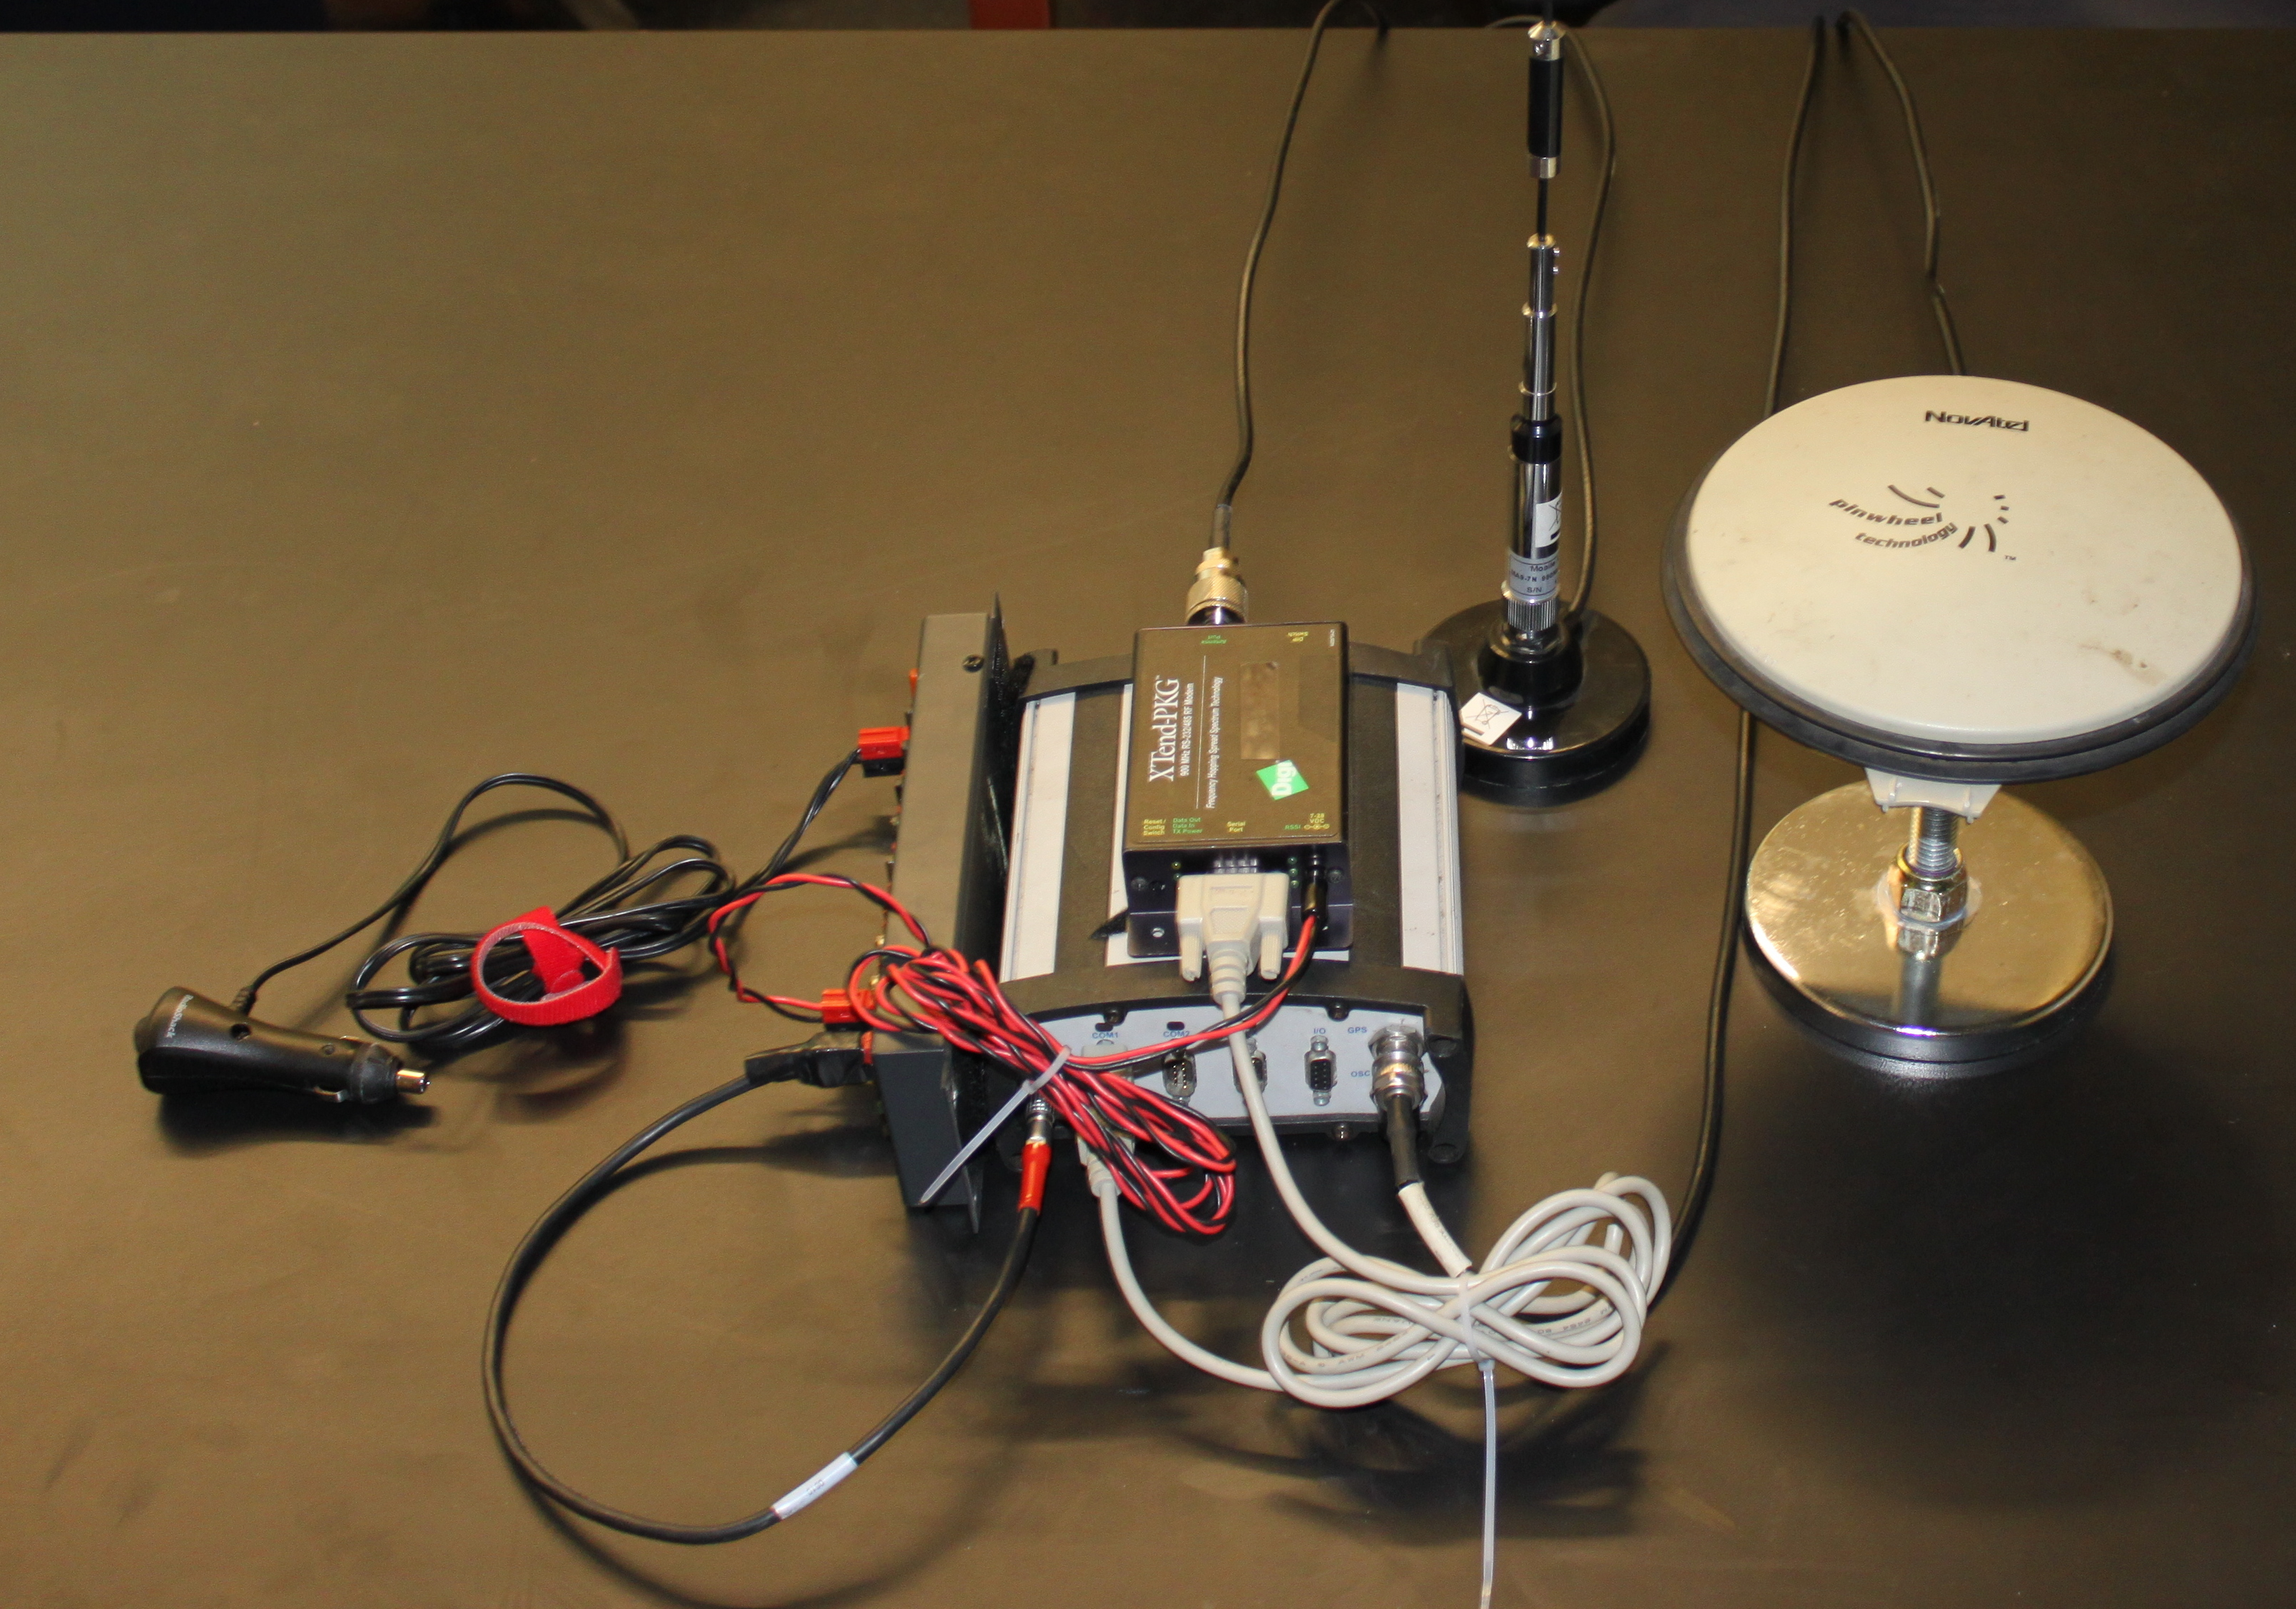
\includegraphics[width=4cm]{../graphics/lead_hardware.jpg}
        \end{figure}
    \end{frame}

    \begin{frame}{Experimentation}
      \begin{figure}[ht] \centering
        \includegraphics[width=5cm] {../graphics/driver_view.jpg}
        \caption{\scriptsize View from the driver's seat}
      \end{figure}
      \vspace{-20pt}
      \begin{itemize} \footnotesize
        \item 3 vehicle platforms used: Infiniti G35 (sedan), Hyndai Sonata (SUV), Chevrolet Corvette (coupe)
        \item 11 individual test drivers
        \item Road friction coefficient values set to $\mu_{warn}=0.5,\mu_{crit}=1.0$
        \item 3 testing procedures, performed with each GUI (and without aid where applicable)
      \end{itemize}
    \end{frame}


  %%% Lane Change Test %%%
  \subsection{Lane Change Test}

    \begin{frame}{Lane Change Test --- Procedures}
      \vspace{-30pt}
      \begin{figure}
        % \documentclass[10pt]{article}
% \usepackage[utf8]{inputenc}
% \usepackage{pgf,tikz}
% \usetikzlibrary{arrows}
% \pagestyle{empty}
% \begin{document}

\definecolor{ttzzqq}{rgb}{0.2,0.6,0}
\definecolor{qqqqcc}{rgb}{0,0,0.8}
\definecolor{ffcctt}{rgb}{1,0.8,0.2}
\definecolor{ffzzqq}{rgb}{1,0.2,0}


\begin{tikzpicture}[
    scale=0.3,
    line cap=round,
    line join=round,
    >=triangle 45,
    x=1.0cm,y=1.0cm
    ]

    \begin{scope}[shift={(0,-15)}]

    \clip(-0.94,-2.06) rectangle (29.18,16.12);
    \draw [line width=5.2pt] (16,10)-- (2,10);
    \draw [line width=5.2pt] (16,14)-- (2,14);
    \draw [line width=5.2pt] (14,6)-- (16,6);
    % center stripe
    \draw [shift={(16,8)},line width=3pt,dash pattern=on 5pt off 5pt,color=ffcctt]  plot[domain=-1.57:1.57,variable=\t]({1*4*cos(\t r)+0*4*sin(\t r)},{0*4*cos(\t r)+1*4*sin(\t r)}); 
    \draw [line width=3pt,dash pattern=on 5pt off 5pt,color=ffcctt] (14,4)-- (16,4);
    \draw [line width=3pt,dash pattern=on 5pt off 5pt,color=ffcctt] (16,12)-- (4,12);

    \draw [shift={(16,8)},line width=5.2pt]  plot[domain=-1.57:1.57,variable=\t]({1*6*cos(\t r)+0*6*sin(\t r)},{0*6*cos(\t r)+1*6*sin(\t r)});
    \draw [shift={(16,8)},line width=5.2pt]  plot[domain=-1.57:1.57,variable=\t]({1*2*cos(\t r)+0*2*sin(\t r)},{0*2*cos(\t r)+1*2*sin(\t r)});
    \draw [line width=5.2pt] (16,2)-- (14,2);
    % path
    \draw [shift={(13.19,10.74)},line width=2pt,dotted,color=qqqqcc]  plot[domain=1.61:2.63,variable=\t]({1*2.58*cos(\t r)+0*2.58*sin(\t r)},{0*2.58*cos(\t r)+1*2.58*sin(\t r)});
    \draw [shift={(8.37,13.37)},line width=2pt,dotted,color=qqqqcc]  plot[domain=4.97:5.79,variable=\t]({1*2.91*cos(\t r)+0*2.91*sin(\t r)},{0*2.91*cos(\t r)+1*2.91*sin(\t r)});
    \draw [line width=2pt,dotted,color=qqqqcc] (13.08,13.32)-- (16.04,13.24);
    \draw [shift={(16,8.05)},line width=2pt,dotted,color=qqqqcc]  plot[domain=-1.58:1.56,variable=\t]({1*5.19*cos(\t r)+0*5.19*sin(\t r)},{0*5.19*cos(\t r)+1*5.19*sin(\t r)});

    \begin{scriptsize}
        % cones
        \fill [color=ffzzqq] (4,12)     circle (5.0pt);
        \fill [color=ffzzqq] (6,12)     circle (5.0pt);
        \fill [color=ffzzqq] (8,12)     circle (5.0pt);
        \fill [color=ffzzqq] (10,12)    circle (5.0pt);
        \fill [color=ffzzqq] (12,12)    circle (5.0pt);
        \fill [color=ffzzqq] (14,12)    circle (5.0pt);
        % leader
        \fill [color=ttzzqq,shift={(9.12,10.56)},rotate=90] (0,0) ++(0 pt,6.75pt) -- ++(5.85pt,-10.125pt)--++(-11.69pt,0 pt) -- ++(5.85pt,10.125pt);
        \draw[color=ttzzqq] (8,11) node {$Leader$};
        % follower
        \fill [color=ttzzqq,shift={(15.96,2.86)},rotate=270] (0,0) ++(0 pt,6.75pt) -- ++(5.85pt,-10.125pt)--++(-11.69pt,0 pt) -- ++(5.85pt,10.125pt);
        \draw[color=ttzzqq] (14.5,3.32) node {$Follower$};
    \end{scriptsize}

    \end{scope}

\end{tikzpicture}


% \end{document}
      \end{figure}
      \vspace{-40pt}
      \begin{itemize} \small
        \item Lane change maneuver is visually obscured from follower.
        \item Following driver signalled to begin once maneuver completed.
        \item 6 cones spaced at $\approx10m$.
        \item Results treated as pass/fail.
      \end{itemize}
      % text describing test
    \end{frame}
    
    % What the drivers saw in each GUI during the lane change
    \begin{frame}{Lange Change Test --- Driver View}
      \begin{figure}[ht] \centering
        \begin{minipage}[b]{0.45\linewidth} \centering 
          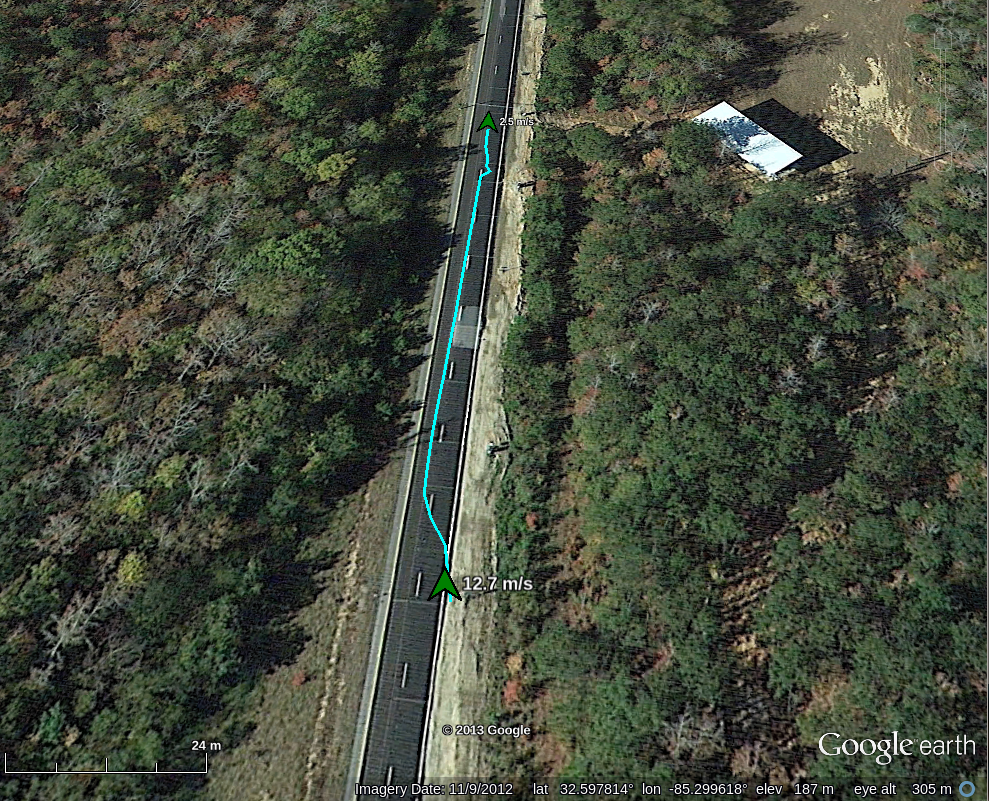
\includegraphics[width=\textwidth]{../graphics/lane_change.png}
          \caption{Google Earth GUI approaching the lane change maneuver}
        \end{minipage}
        \hspace{0.5cm}
        \begin{minipage}[b]{0.45\linewidth} \centering
          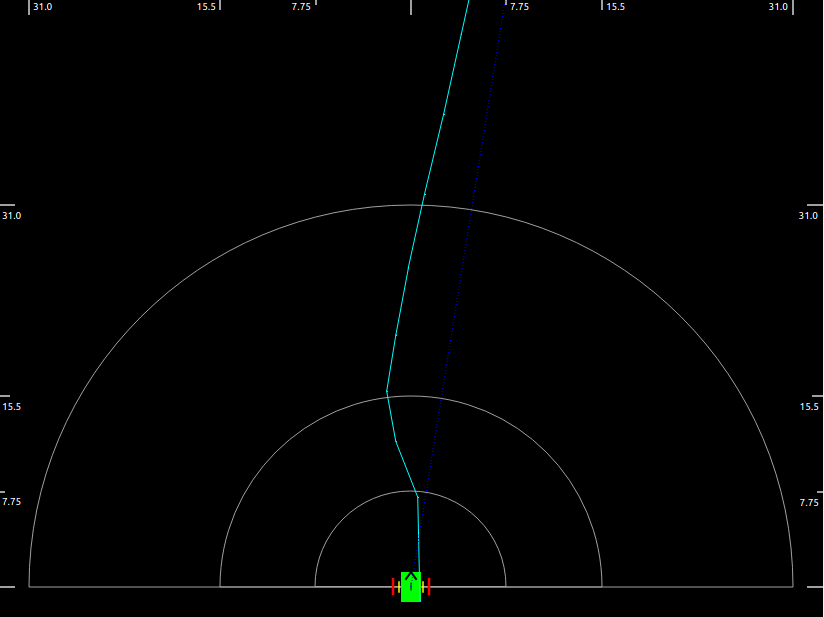
\includegraphics[width=\textwidth]{../graphics/lane_change_mono.png} 
          \caption{Qt GUI approaching the lane change maneuver}
        \end{minipage}
      \end{figure}
    \end{frame}

    % present data
    \begin{frame}{Lane Change Test --- Results}
      \begin{itemize} \footnotesize
        \item Ran test 10 times with 4 drivers
        \item Cone placement and start/end points remained constant
        \item Runs eliminated in which driver 
      \end{itemize}
      \vspace{-10pt}
      \begin{table}[htbp] \centering \footnotesize
        % \caption{Cone pairs chosen in the lane change replication test}
        \begin{tabular}{rc|cc}
          GUI&    Run \#  &     Leader&    Follower \\\hline\hline
          Earth&      1       &       1   &    3 \\
               &      2       &       3   &    4 \\ \hline
          Qt   &      3       &       2   &    3 \\
               &      4       &       5   &    5 \\ \hline   
        \end{tabular}
        \label{tab:lanechangeresults}
      \end{table}
      \begin{itemize} \footnotesize
        \item Drivers reported path appeared to be erroneous relative to satellite imagery (e.g., off the road).
        \item Google Earth positioning errors found to vary up to $50m$ \citeitem{ge_accuracy}.
        \item Typically low speeds when deciding where to turn $(<10m/s)$
      \end{itemize}
    \end{frame}


  %%% Precision Following Test %%%

  \subsection{Precision Foll. Test}

    \begin{frame}{Precision Following Test --- Procedures}
      \begin{figure}
        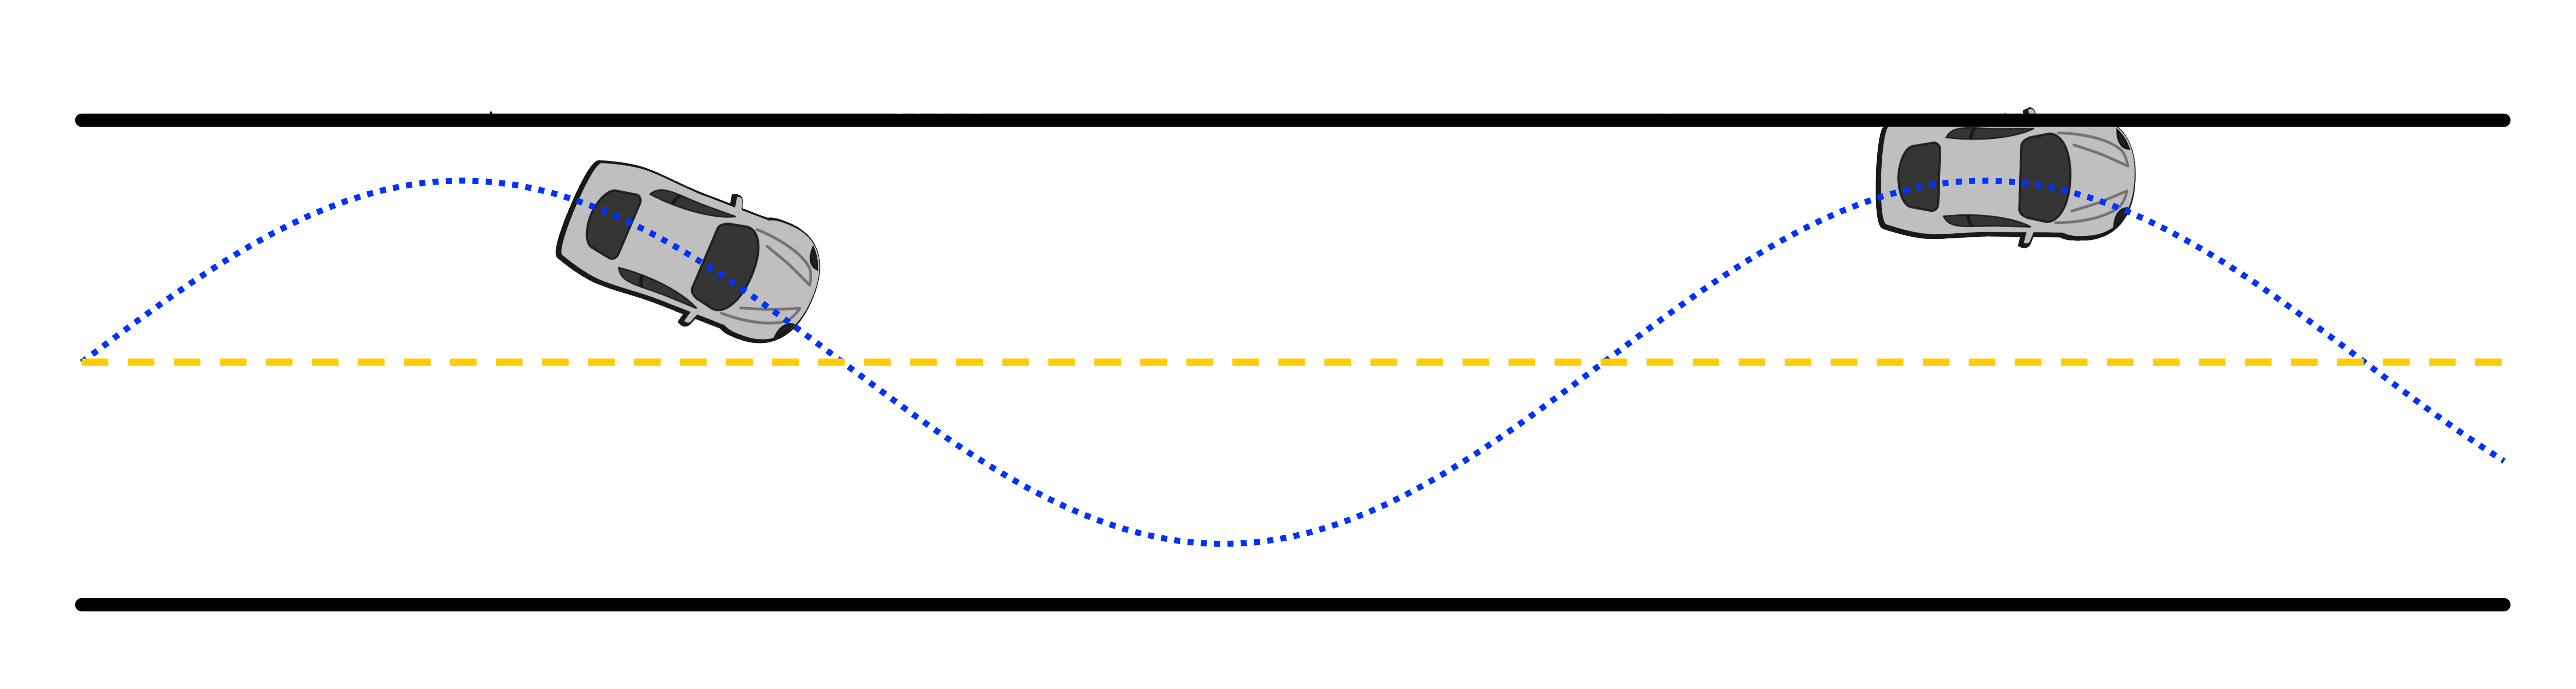
\includegraphics[width=10cm]{../graphics/precision_following_diagram.png}
      \end{figure}   
      \begin{itemize} \footnotesize
        \item Two-lane track similar to 
        \item Performed with each GUI individually, and without aid as control
        \item Run with fewest combined alerts selected as `best' for each.
      \end{itemize}
    \end{frame}

    % present data
    \begin{frame}{Precision Following Test --- Results}
      \begin{columns}
        \begin{column}{0.5\textwidth}
          \begin{figure}
            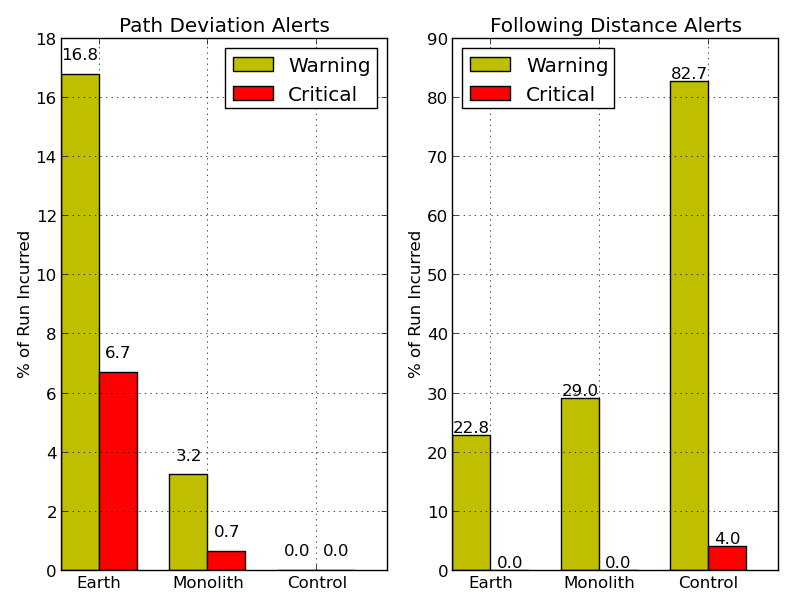
\includegraphics[width=\textwidth]{../graphics/precision_following_alert_percents.png}
          \end{figure}
            % discuss results from both
          \begin{itemize}
            \item Kernel smoothed PDF estimates.
            \item 
            \item 
          \end{itemize}
        \end{column}
        \begin{column}{0.5\textwidth}
          \begin{figure}
            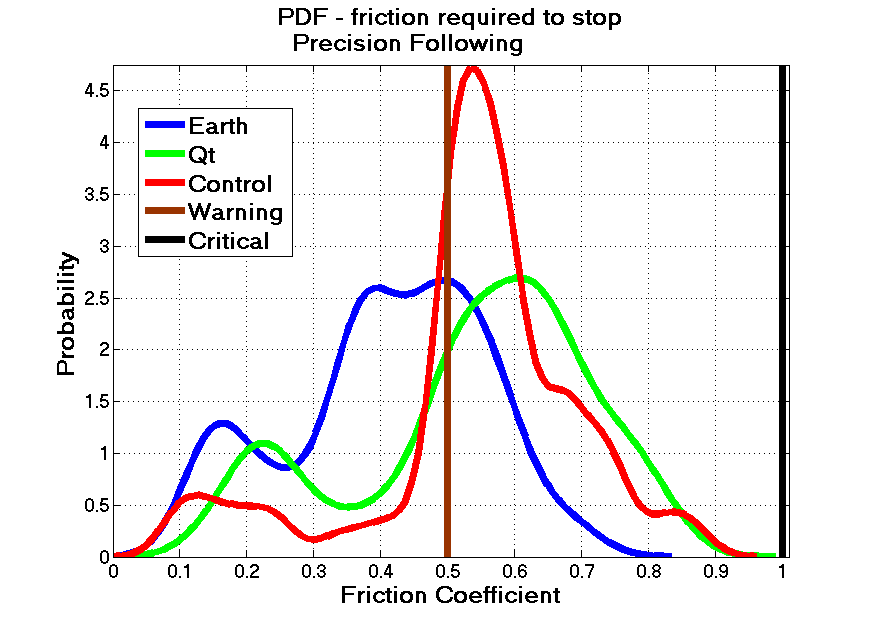
\includegraphics[width=\textwidth]{../graphics/precision_following_mu_distribution.png}
            % \caption{$\mu$ PDF's for best runs}
          \end{figure}
          \vspace{-20pt}
          \begin{figure}
            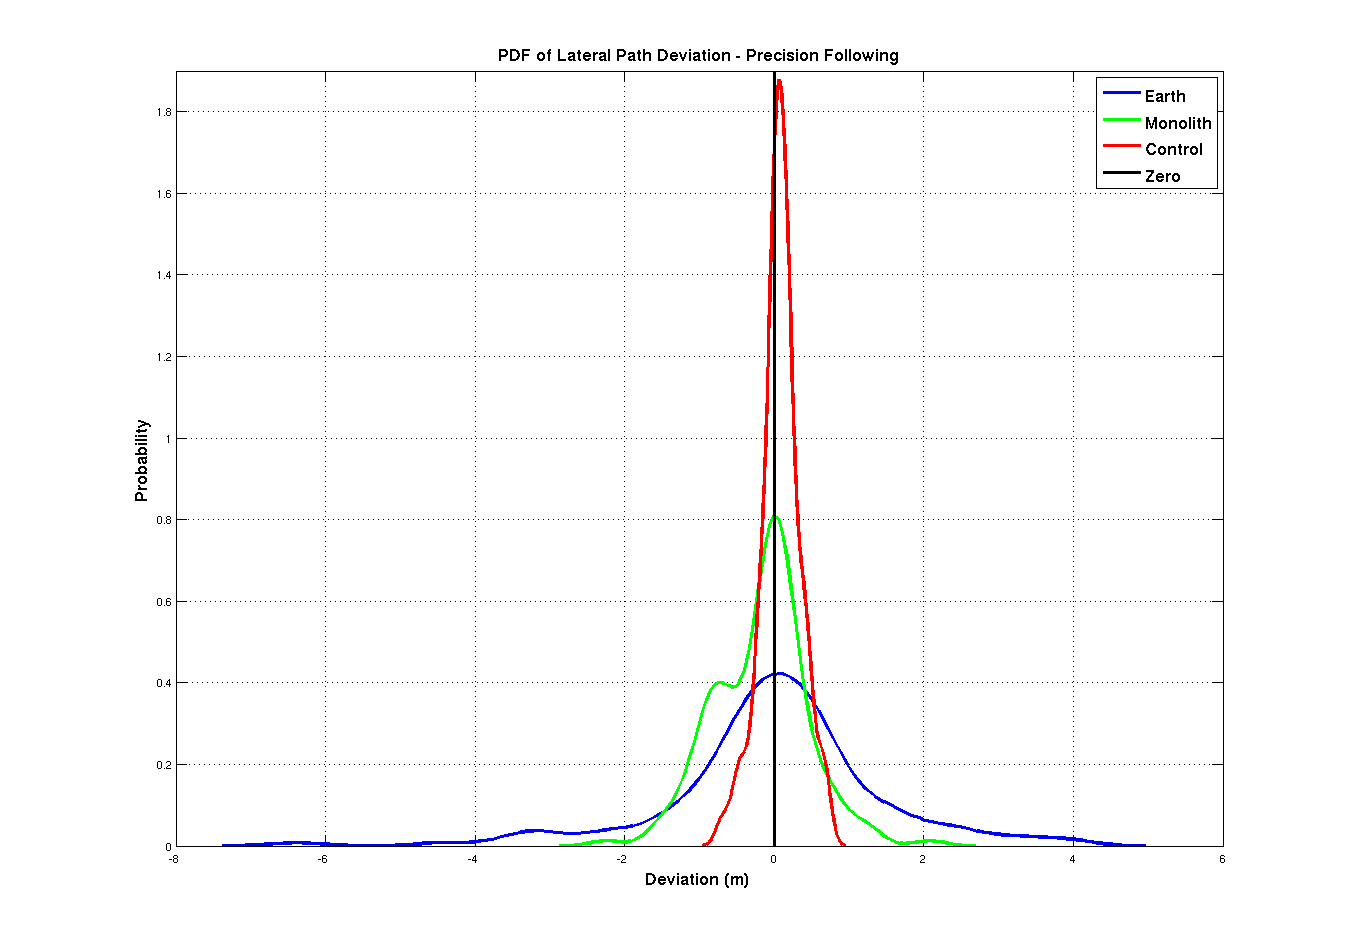
\includegraphics[width=\textwidth]{../graphics/precision_following_dev_pdf.png}
          \end{figure}
        \end{column}
      \end{columns}
    \end{frame}

    % present data
    \begin{frame}{Precision Following Test --- Discussion}
    \end{frame}

  %%% Zero Landmark Test %%%

  \subsection{Zero Landmark Test}
    \begin{frame}{Zero Landmark Test --- Procedures}
      % \vspace{-20pt}
      \begin{itemize}
        \item No lane markings
        \item Wide, open expanse of asphalt
        \item Conducted at night --- minimized visual cues
      \end{itemize}
      \begin{figure}
        \centering
        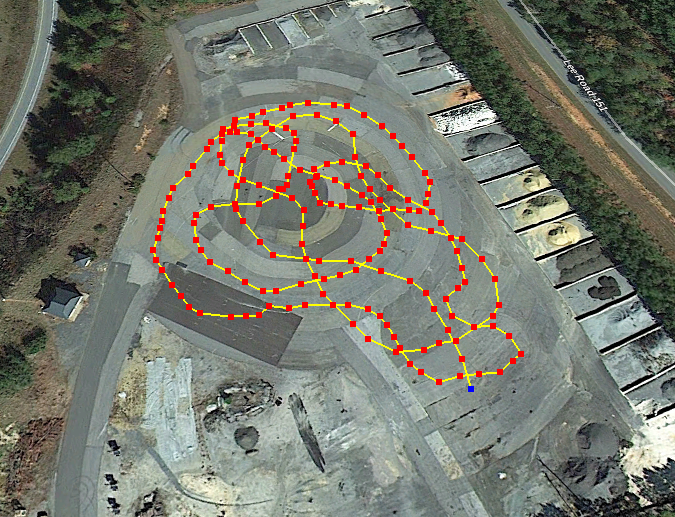
\includegraphics[width=0.55\textwidth]{../graphics/zero_landmark_path.png}
      \end{figure}     
    \end{frame}

    % present data
    \begin{frame}{Zero Landmark Test --- Results}
      \begin{columns}
        \begin{column}{0.5\textwidth}
          \begin{figure}
            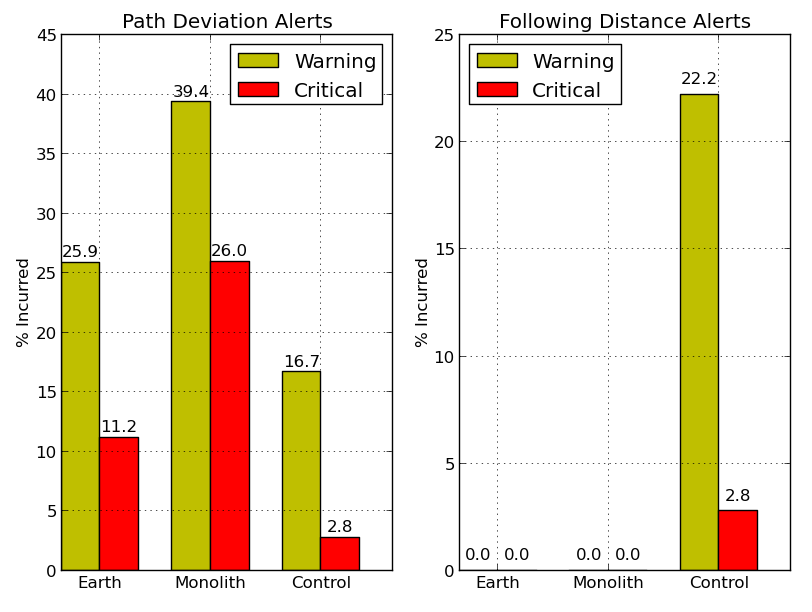
\includegraphics[width=\textwidth]{../graphics/zero_landmark_alert_percents.png}
          \end{figure}
            % discuss results from both
          \begin{itemize} \scriptsize
            \item Kernel smoothed PDF estimates.
            \item 
            \item 
          \end{itemize}
        \end{column}
        \begin{column}{0.5\textwidth}
          \begin{figure}
            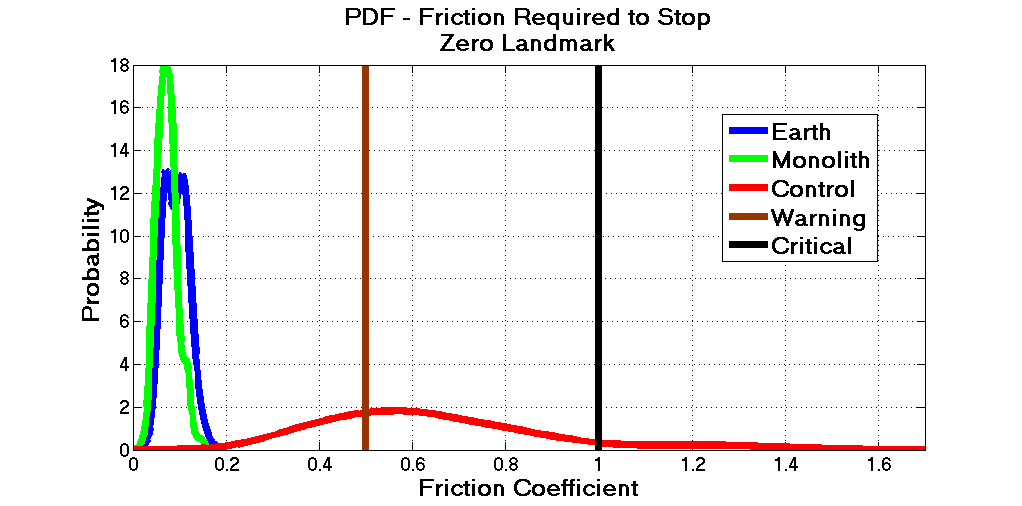
\includegraphics[width=\textwidth]{../graphics/zero_landmark_mu_distribution.png}
            % \caption{$\mu$ PDF's for best runs}
          \end{figure}
          \vspace{-20pt}
          \begin{figure}
            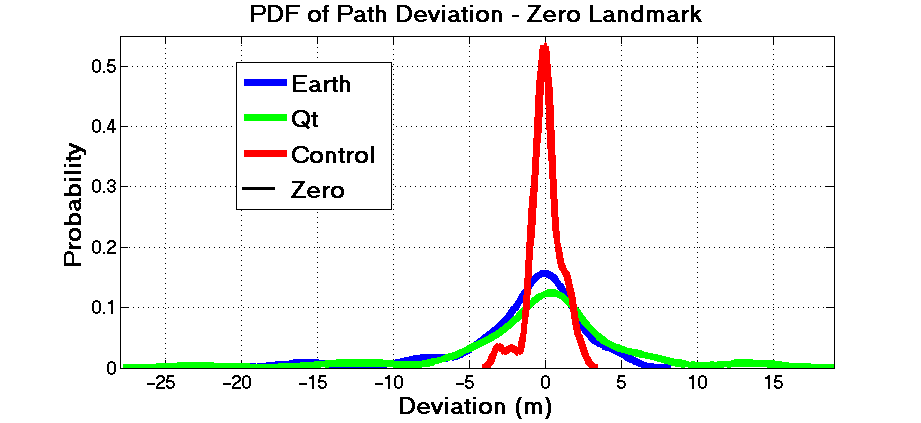
\includegraphics[width=\textwidth]{../graphics/pdf_zero_landmark_deviation.png}
          \end{figure}
        \end{column}
      \end{columns}
    \end{frame}

    % what happened
    \begin{frame}{Zero Landmark Test --- Discussion}
    \end{frame}



%%%%%%%%%%%%%%%%
%% Conclusion %%
%$%%%%%%%%%%%%%%
\section{Conclusion}

  \begin{frame}{Future Work}
    \begin{itemize}
      \item Reduce latency in combined system
      \item 
    \end{itemize}
  \end{frame}

\end{document}




%%%%%%%%%%%%%%%%%%%%%%%%%%%%%%%%%%%%%%%%%%%%%%%%%%%%%%%%%%%%%%%%%%%%%%%%%%%%%%%%

%% Font Sizes
% \tiny
% \scriptsize
% \footnotesize
% \small
% \normalsize
% \large
% \Large
% \LARGE
% \huge
% \Huge